\chapter{premier chapitre}
	
\section{Exemples dont le titre dans la table des matieres doit etre sur deux lignes} 

\subsection{citations} 

Ceci est un premier exemple de citation \cite{Ful83}. Ceci est un deuxième exemple de citation \citep{GMP81}. Ceci est un troisième exemple de citation \citet{PP98}.

\subsection{acronymes} 

Exemple de définition d'un acronyme de trois lettres : \ac{TLA}. Puis utilisation de cet acronyme en version courte \acs{TLA}.

\subsection{equations}   

\begin{equation}
E=mc^2	
\end{equation}

\subsection{figures}   

Lorem ipsum dolor sit amet, consectetur adipisicing elit, sed do eiusmod
tempor incididunt ut labore et dolore magna aliqua. Ut enim ad minim veniam,
quis nostrud exercitation ullamco laboris nisi ut aliquip ex ea commodo
consequat.

Lorem ipsum dolor sit amet, consectetur adipisicing elit, sed do eiusmod
tempor incididunt ut labore et dolore magna aliqua. Ut enim ad minim veniam,
quis nostrud exercitation ullamco laboris nisi ut aliquip ex ea commodo
consequat.

\begin{figure}[H]
 \centering
 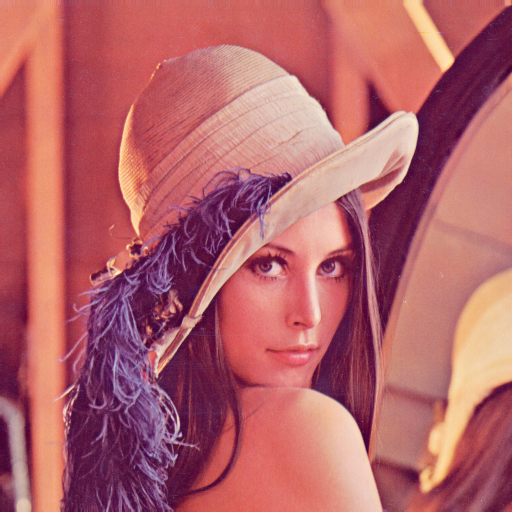
\includegraphics[width=7cm]{lenna.png}
 \caption{Titre de la figure qui doit normalement se tenir sur deux lignes car il est assez long}
 \label{fig:figure1}
\end{figure}

Lorem ipsum dolor sit amet, consectetur adipisicing elit, sed do eiusmod
tempor incididunt ut labore et dolore magna aliqua. Ut enim ad minim veniam,
quis nostrud exercitation ullamco laboris nisi ut aliquip ex ea commodo
consequat.

Lorem ipsum dolor sit amet, consectetur adipisicing elit, sed do eiusmod
tempor incididunt ut labore et dolore magna aliqua. Ut enim ad minim veniam,
quis nostrud exercitation ullamco laboris nisi ut aliquip ex ea commodo
consequat.

\subsection{tableaux}   

Lorem ipsum dolor sit amet, consectetur adipisicing elit, sed do eiusmod
tempor incididunt ut labore et dolore magna aliqua. Ut enim ad minim veniam,
quis nostrud exercitation ullamco laboris nisi ut aliquip ex ea commodo
consequat.

\begin{table}[H]
  \begin{center}
    \caption{Titre du tableau qui doit normalement se tenir sur deux lignes}
    \label{tab:table1}
    \begin{tabular}{l|c|r}
      \textbf{Value 1} & \textbf{Value 2} & \textbf{Value 3}\\
      $\alpha$ & $\beta$ & $\gamma$ \\
      \hline
      1 & 1110.1 & a\\
      2 & 10.1 & b\\
      3 & 23.113231 & c\\
    \end{tabular}
  \end{center}
\end{table}

Lorem ipsum dolor sit amet, consectetur adipisicing elit, sed do eiusmod
tempor incididunt ut labore et dolore magna aliqua. Ut enim ad minim veniam,
quis nostrud exercitation ullamco laboris nisi ut aliquip ex ea commodo
consequat.